\documentclass{IEEEtran}
\usepackage{amsmath}
\usepackage{graphicx}
\usepackage{color}
%\usepackage{circuitikz}
\begin{document}
\title{A 28-nm Bulk CMOS Quantum Controller Achieving }
\author{Joseph~C.~Bardin, \emph{Senior Member, IEEE}, Evan~Jeffrey, Erik~Lucero, Trent~Huang, Sayan~Das,~\emph{Student Member, IEEE}, Ofer~Naaman, Rami~Barends, Ted~White, Marissa~Giustina, Daniel~Sank, Pedram~Roushan, Kunal~Arya, Benjamin~Chiaro, Julian~Kelly, Jimmy~Chen, Brian~Burkett, Yu~Chen, Andrew~Dunsworth, Austin~Fowler, Brooks~Foxen, Craig~Gidney, Rob~Graff, Paul~Klimov, Josh~Mutus, Matthew~McEwen, Anthony~Megrant, Matthew~Neeley, Charles~Neill, Chris~Quintana, Amit~Vainsencher, Hartmut~Neven, and John~Martinis}
\maketitle
\begin{abstract}
A
\end{abstract}

\section{Introduction}

\section{Transmon qubit controller requirements}
\subsection{Quantum Control}
In quantum computing, 

Prior to describing circuits, it is important to quantify the hardware requirements for quantum control. 

\subsection{Control of a Transmon}

\begin{equation}
\hat{H}=\left[\right]
\end{equation}
\subsection{XY Controller Requirements}
\subsubsection{Physical Temperature}
\subsubsection{Power Consumption}
Currently no multiplexing, however such functionality would relax power consumption.
\subsubsection{Signal Levels}
\subsubsection{ON/OFF Ratio}
\subsubsection{Gate Fidelity}
As achieving fault-tolerance is a long term goal of the quantum computing community, it is important that the gates carried out using a  
\begin{figure}[bt!]
\includegraphics[width=\columnwidth]{Figures/CONCEPT_FULL}
\caption{\color{red}Chip block diagram}
\end{figure}
\begin{figure}[bt!]
\includegraphics[width=\columnwidth]{Figures/CHIP_BLOCK_DIAGRAM}
\caption{\color{red}Chip block diagram}
\end{figure}
\begin{figure}
\includegraphics[width=\columnwidth]{Figures/ENV_DAC}
\end{figure}
\begin{figure}[bt!]
\includegraphics[width=\columnwidth]{Figures/MODULATOR}
\caption{\color{red}Chip block diagram}
\end{figure}
\begin{figure}[bt!]
\includegraphics[width=\columnwidth]{Figures/timedomainfig}
\caption{\color{red}Chip block diagram}
\end{figure}
\begin{figure}[bt!]
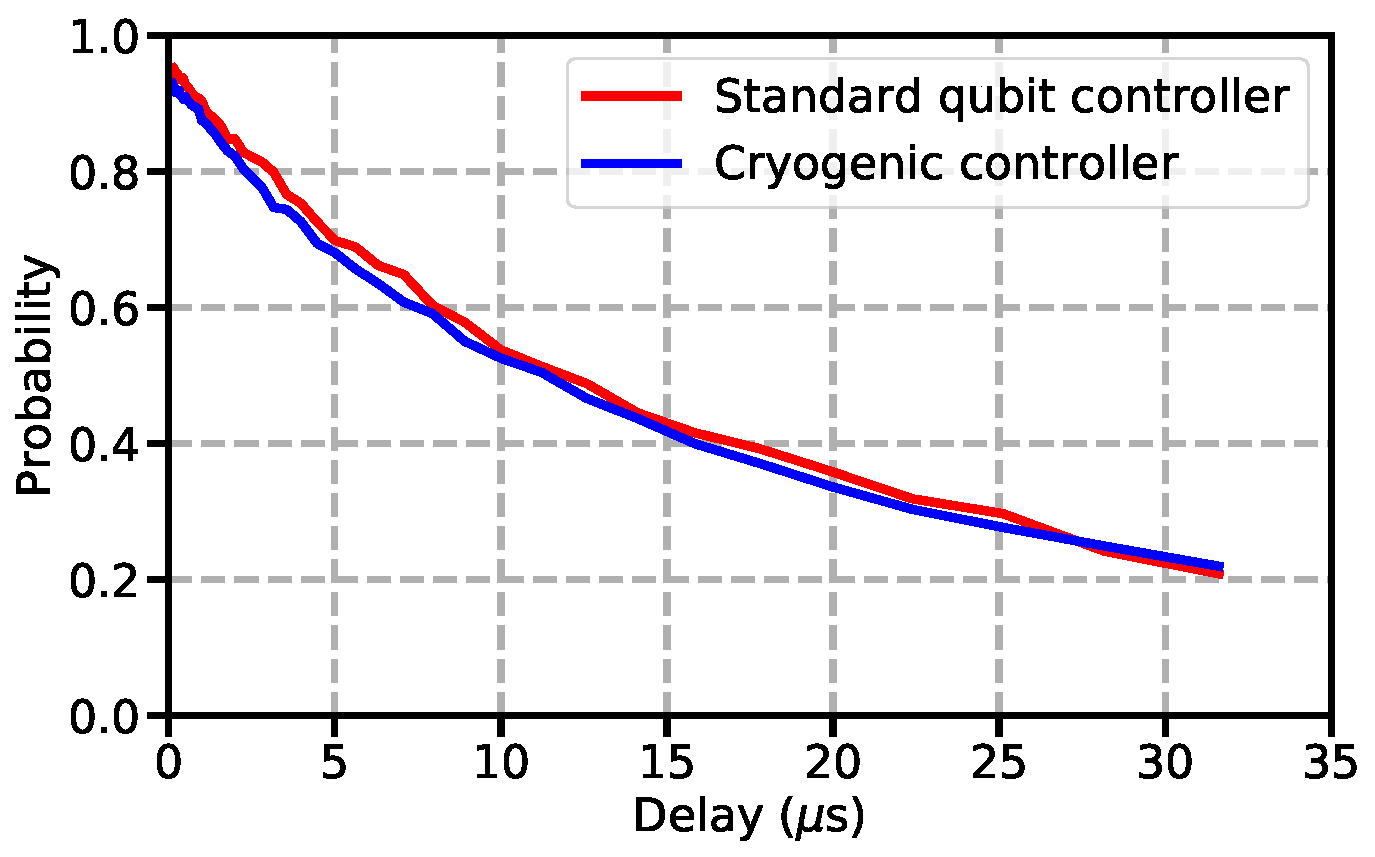
\includegraphics[width=\columnwidth]{Figures/Coherence}
\caption{\color{red}Chip block diagram}
\end{figure}
\begin{figure}[bt!]
\includegraphics[width=\columnwidth]{Figures/twostate_log}
\caption{\color{red}Add limit}
\end{figure}
\begin{figure}[bt!]
\includegraphics[width=\columnwidth]{Figures/RABI_REFORMAT_ONE_RESULT}
\caption{\color{red}Chip block diagram}
\end{figure}
\begin{figure}[bt!]
\includegraphics[width=\columnwidth]{Figures/WAVE_RABI_2}
\caption{\color{red}Chip block diagram}
\end{figure}
\section{Results}
\section{Conclusion}
\end{document}